\section{Installation, Integration, and Commissioning}
\label{sec:dp-pds-installation}

\subsection{Transport and Handling}

\dwords{pmt} will be transported on a standard EUR pallet that is \SI{1.2}{\m} $\times$ \SI{1}{\m}. Figure~\ref{fig:dppd_11_2} shows the largest capacity commercially available box. The box can hold \num{36} \dwords{pmt} in three levels of \num{4} $\times$ \num{3} arrays. Individual \dwords{pmt} will be placed in cartons with their bases, support structures, and short \dword{hv} cables soldered to the bases at the production/assembly sites. For shipping to \dword{ctsf}, \num{36} \dwords{pmt} will then be placed in the transport boxes.

\begin{dunefigure}[An example transportation box to be used for all transport purposes i.e. from remote sites to the \dword{ctsf} and from \dword{ctsf} to \surf.]{fig:dppd_11_2}
{An example transportation box to be used to transport items from remote sites to the \dword{ctsf} and from \dword{ctsf} to \surf.}
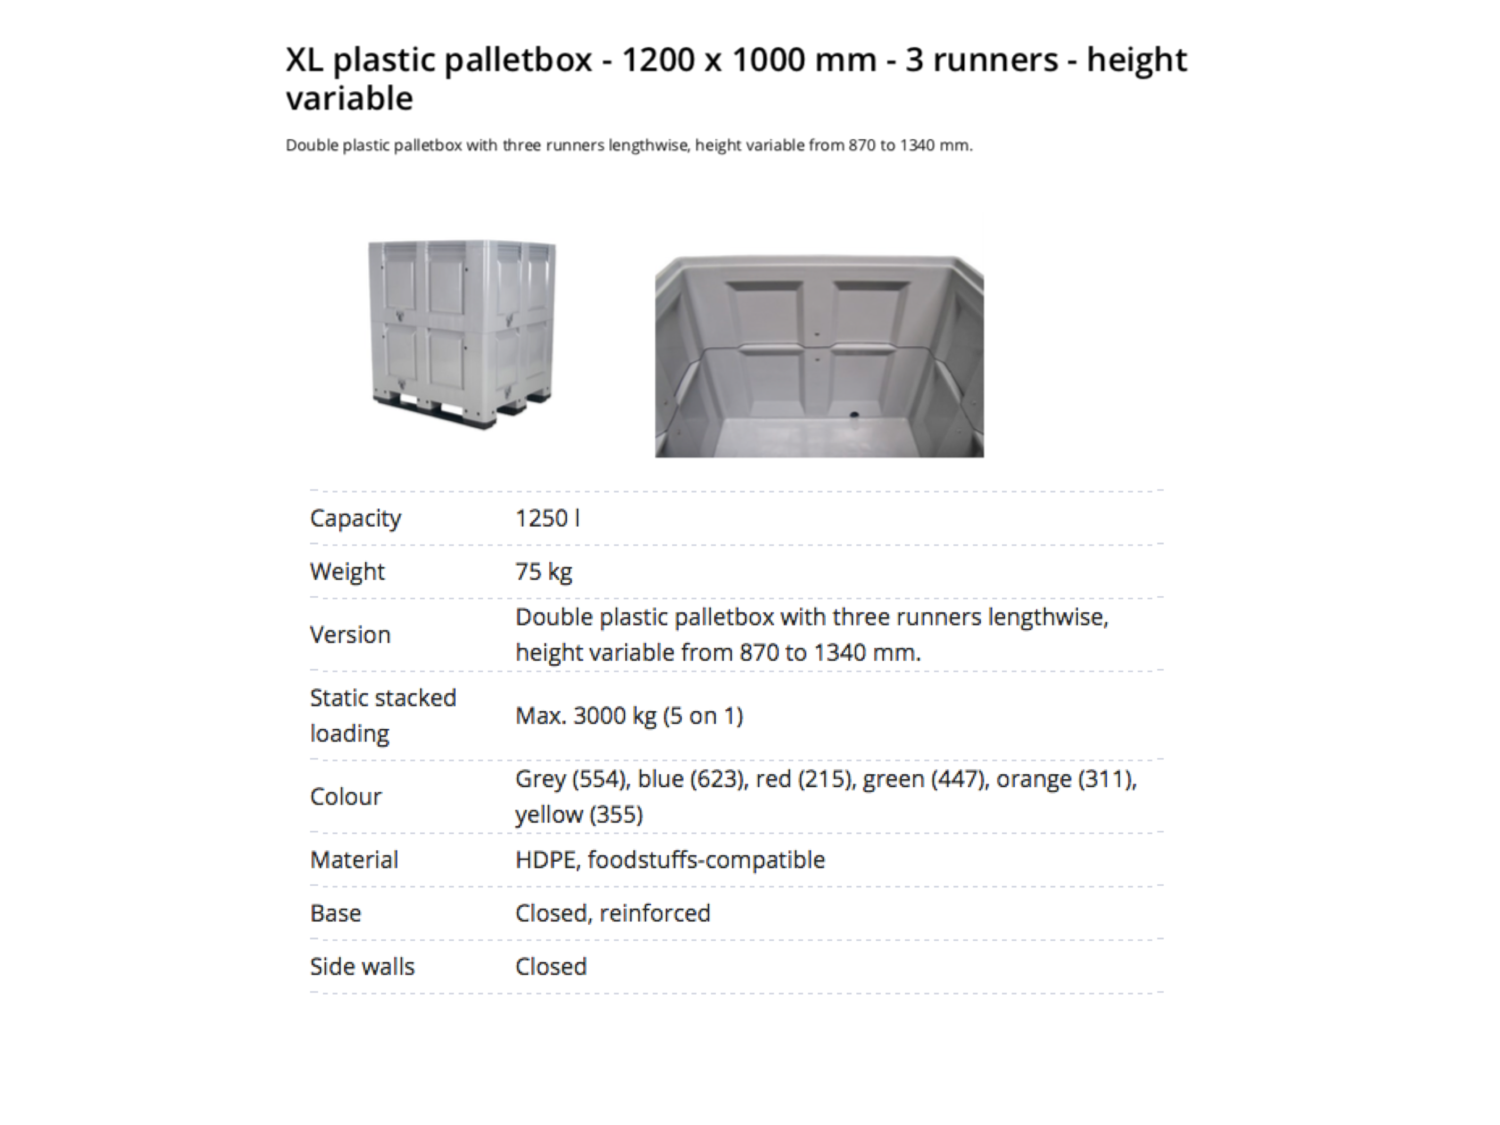
\includegraphics[width=0.5\textwidth]{dppd_11_2}
\end{dunefigure}

Following the \dword{ctsf} operations, the \dwords{pmt} will be placed in a custom structure in \num{4} $\times$ \num{3} arrays. The structure will be assembled with metal and plastic parts so the entire structure, together with the \dwords{pmt}, can be moved into the clean room underground. Three of these structures will be placed on top of each other inside the boxes with the crane. The individual cartons that held the \dwords{pmt} will be recycled at the \dword{ctsf}. The local movement of the transportation boxes in the \dword{ctsf} can be done with compact warehouse forklifts. The \dword{ctsf} will also be used as the storage area for the large \dword{pmt} transportation boxes before they are sent to \surf. The boxes will be stored in single-shelf racks to the right and left of the entrance to the work area (Fig.~\ref{fig:dppd_11_3}). The first set of boxes will be placed on the floor and the second set will be on a shelf that is \SI{1.5}{\m} off the ground. This area can store the entire \dual \dword{pds} \dword{pmt} inventory of \dpnumpmtch \dwords{pmt} in \num{20} boxes. The \num{80} spare \dwords{pmt} can be placed in three boxes, which can be stored on the floor in the available space in the work area as the \dual \dword{pds} \dword{ctsf} operations are finished.

The large \dword{pds} boxes will be wrapped with plastic foil at the \dword{ctsf} that will be opened in \dwords{sas} underground. After removing the plastic wrapping, the transport boxes, with their entire contents, will be moved into the cleanroom. The \dword{pds} boxes can be moved around the underground areas with a pallet jack. Each \num{4} $\times$ \num{3} structure will be removed from the transportation box and moved inside the cleanroom by the crane. The structure will go in the dark box for functionality tests of the \num{12} \dwords{pmt}. The transportation boxes will be used for storage before installation. Empty boxes will be returned to \dword{ctsf}. At most, three \dword{pds} boxes will be in the cleanroom at a time.

The \num{4} $\times$ \num{3} structure will be moved by crane into the cryostat and placed on the cryostat floor at a location convenient to the active installation area. The \dwords{pmt} will then be installed one by one. 

%\subsection{Integration and Testing Facility Operations}
\subsection{Coating, Testing and Storage Facility Operations}
\label{subsec:dp-pds-itf}

The \dword{ctsf} will be \SI{10}{\m} $\times$ \SI{8}{\m} with a (\SI{12}{\ft}) ceiling equipped with a gantry crane. The facility will be used to apply the \dword{tpb} coating on the \dword{pmt} windows, for \dword{qc} of the \dwords{pmt}, and for storage and preparation for transport to \surf. If the option of installing individual ground grids on the \dword{pmt} support structures, which is under consideration by the \dual \dword{pds} and \dword{hv} consortia, is realized, this operation will also be performed at the \dword{ctsf}. The layout of the \dword{ctsf} is shown in Figure~\ref{fig:dppd_11_3}.

\begin{dunefigure}[The layout of the \dword{ctsf}.]{fig:dppd_11_3}
{The layout of the \dword{ctsf}.}
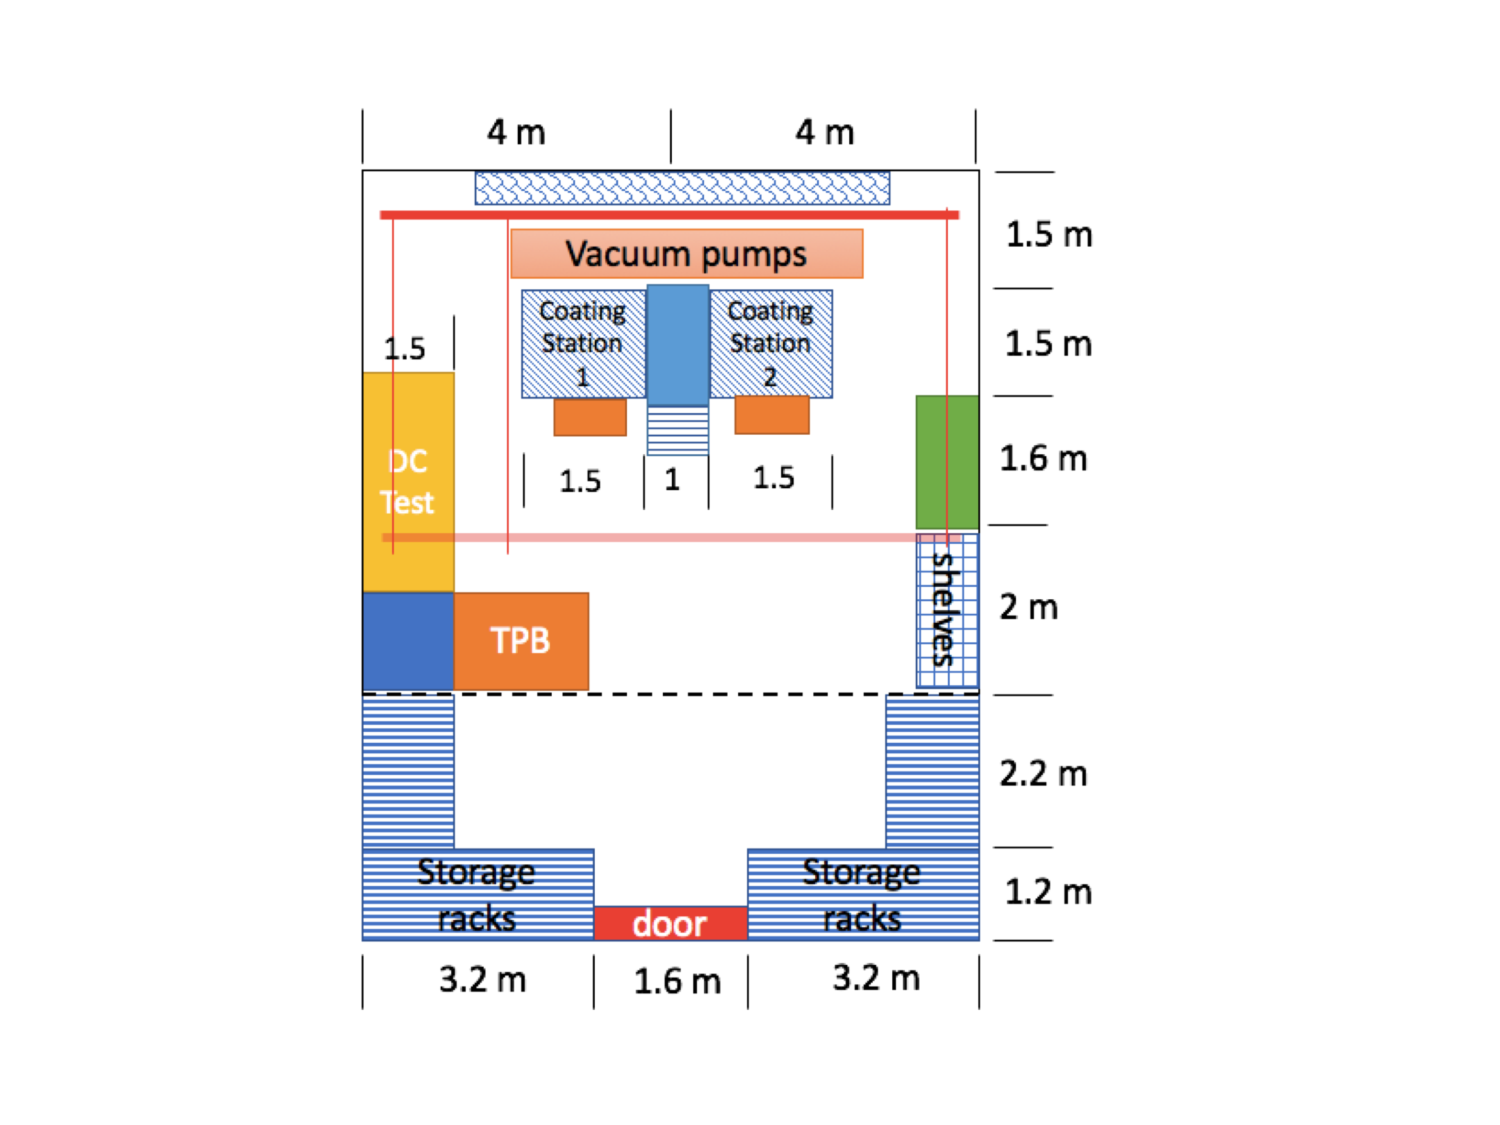
\includegraphics[width=0.4\textwidth]{dppd_11_3}
\end{dunefigure}

Two coating stations will be \SI{1.5}{\m} $\times$ \SI{1.5}{\m}. Figure ~\ref{fig:dppd_11_4} shows pictures of a \dword{tpb} coating station at the \dword{cern} thin film facility. Between the two coating stations, an elevated platform, accessible by stairs, will be placed. This platform will be used to reach the top of the evaporator (approximately \SI{1.5}{\m} high from the ground level) and inside the vessel. Cooling water, nitrogen, and electricity will be provided from the outlets placed along the \SI{8}{\m} wall (indicated with wavy lines in Figure~\ref{fig:dppd_11_3}). Vacuum pumps will be placed in the immediate vicinity of the evaporators. Control electronics will also be placed next to the evaporator chambers. 

\begin{dunefigure}[Pictures of a single \dword{tpb} coating station (courtesy of Wil Vollenberg, \dword{cern}-TE Department).]{fig:dppd_11_4}
{Pictures of a single \dword{tpb} coating station (courtesy of Wil Vollenberg, \dword{cern}-TE Department).}
\includegraphics[width=0.8\textwidth]{dppd_11_4}
\end{dunefigure}

The \dwords{pmt} will be taken out of their individual cartons when they arrive at the \dword{ctsf}. The \dwords{pmt} will first be tested for basic functionality in their cartons to verify that they have been safely transported from the remote sites and will be kept in these boxes until the windows are coated. The \dword{pmt} windows will be cleaned with acetone and isopropanol before the evaporation. This will be done in the flow device/fume hood shown as a green box along the \SI{10}{\m} wall in Fig.~\ref{fig:dppd_11_3}. The gantry crane (indicated with red bars in Fig.~\ref{fig:dppd_11_3}) can move parts between the coating stations and the work desks. It will be used to remove the vessel lid and support it while the \dword{pmt} is installed for coating.

Following the evaporation procedure, an acrylic protective plates will be installed to cover the coated \dword{pmt} windows.
%, and the \dwords{pmt} will be placed in individual dark plastic protective bags. 
The \dwords{pmt} will be tested again for basic functionality. They will then be attached to the \num{4} $\times$ \num{3} structure for transportation to \surf.

At the \dword{ctsf}, the \dword{pmt} windows will be coated at a rate of \num{4} \dwords{pmt}/day or \num{20} \dwords{pmt}/week and \num{80} \dwords{pmt}/month. Given the installation rate of \num{120} \dwords{pmt}/month, the \dword{ctsf} operations should start before installation begins. \dword{ctsf} has sufficient storage capacity for the entire \dword{pmt} inventory of the \dword{pds}. 

\subsection{Underground Installation and Integration}
\label{subsec:dp-pds-undergroundinstallation}

The cryostat cable/fiber installation will precede the installation of the \dword{fc}. The cables/fibers will be routed from the flanges to the bottom of the cryostat. The total cable/fiber mass (length) is approximately \SI{50}{\kg} (\SI{25}{\m}) per sector with an average mass/length of \SI{2}{\kg/\m}, where one sector comprises \num{36} \dwords{pmt} (see Section~\ref{sec:dp-pds-overview_layout}). The free ends of the cables/fibers will be temporarily attached to the cryostat floor so they can be easily accessed during installation. The cable/fiber and tray installation will be done on both sides of the cryostat. At this stage, the \dword{hv} cables will be transported in a single box from the \dword{ctsf} to \surf. At the same time, a separate box containing \num{120} calibration fiber + fiber bundle assemblies will be transported from the \dword{ctsf} to \surf. The boxes will be transported to the cryostat roof so the cables/fibers can be hung through the feedthroughs for installation in the cable trays.  

Once the plastic wrap is removed, the \dword{pds} \dword{pmt} box and its entire contents can be moved to the clean room. The \dwords{pmt} will undergo functionality tests inside the custom design dark box, which can cover the entire structure of \num{4} $\times$ \num{3} \dwords{pmt}. The dark box will have a high voltage patch panel and allow consecutive tests of all \num{12} \dwords{pmt} in one testing session without intervention. The test will be a simple check for healthy \dword{pmt} operations. Once the operation of the \dwords{pmt} is verified, the structure can be moved into the cryostat.

Inside the cryostat, the \dwords{pmt} will be removed from the structure. %The window protections will be kept on the \dwords{pmt}. 
The \dwords{pmt} will be mounted on the membrane floor in the areas between the membrane corrugations using their support structures. The attachment is done using a stainless steel support base that can be point-glued to the membrane. The weight of the support and the \dword{pmt} exceeds the buoyancy force of the system. Furthermore, these supports also ensure stability against possible lateral forces acting on the \dwords{pmt} due to the liquid flow. Once the attachment is complete, the short \dword{hv} cables will be connected to the cold \dword{hv} cables with SHV barrel connectors. The calibration fibers will be routed and connected to the support structure. Once all the \dwords{pmt} of a given \dword{pds} sector are installed, the cables and fibers will be fixed in their final positions.

The installation will be done at a rate of \num{30} \dwords{pmt}/week. After installation, the empty \dword{pmt} boxes and the transport structures will be taken back to \dword{ctsf}.

Table~\ref{tab:dppd_t_11_1} summarizes the quantities related to the \dual \dword{pds} installation.

\begin{dunetable}
[Quantities related to the \dual \dword{pds} installation.]
{lc p{0.8\textwidth}}
{tab:dppd_t_11_1}
{Quantities related to the \dual \dword{pds} installation.}
Parameter & Value \\
Number of \dual \dword{pds} sectors	& \num{20} \\
Number of \dwords{pmt} per sector	& \num{36} \\
Number of calibration fibers per sector	& \num{6} \\
Number of feedthrough flanges per sector	& \num{1} \\
Total number of feedthrough flanges	& \num{20} \\
Number of \dword{hv} racks per sector	& \num{1} \\
Frequency of transportations to \surf from \dword{ctsf}	& \num{4} \dword{pds} boxes per month \\
Rate of installation	& \num{30} \dwords{pmt}/week \\
\end{dunetable}

The reflector/\dword{wls} panels will be assembled into a unit panel assembly on a dedicated table underground immediately prior to the installation following the procedure described in Section \ref{sec:dp-pds-mechanics}. They will be placed in a storage structure that can hold three regular and two extended reflector/\dword{wls} panel assemblies to be installed in one row of an \dword{fc} super-module. The installation of the panel assemblies will be synchronized with the installation of the \dword{fc} modules, which is described in Section \ref{sec:fddp-hv-transport-install} and depicted in Fig. ~\ref{fig:dp-super-module-installation-secuence}. Once a row of the \dword{fc} super-module is installed, the five reflector/\dword{wls} panel assemblies will be mounted on the FRP I-beams of the \dword{fc} submodules, starting from one end of the row and progressing towards the other. Figure \ref{fig:dppd_reflective_panel_installation_sequence} depicts the installation sequence of a unit reflector/\dword{wls} panel. The sequence can be described as below:

\begin{enumerate}
\item Put the top two screws accessing the back side through the top liquid flow opening (Fig.~ \ref{fig:dppd_reflective_panel_installation_sequence}  left).
\item Place two nuts in the closed holes of the long holding bar. Slide the long bar behind the panel to the level of the middle bar by holding it through the central liquid flow opening. Put the two middle bar screws and remove the long bar through the bottom liquid flow opening after sliding it all the way down (Fig.~ \ref{fig:dppd_reflective_panel_installation_sequence}  center).
\item Put the bottom two screws accessing the back side through the bottom liquid flow opening (Fig.~ \ref{fig:dppd_reflective_panel_installation_sequence}  right).
\end{enumerate}

\begin{dunefigure}[The schematic view of the installation sequence of a unit reflector/\dword{wls} panel assembly on the \dword{fc} I-beams.]{fig:dppd_reflective_panel_installation_sequence}
{The schematic view of the installation sequence of a unit reflector/\dword{wls} panel assembly on the \dword{fc} I-beams.}
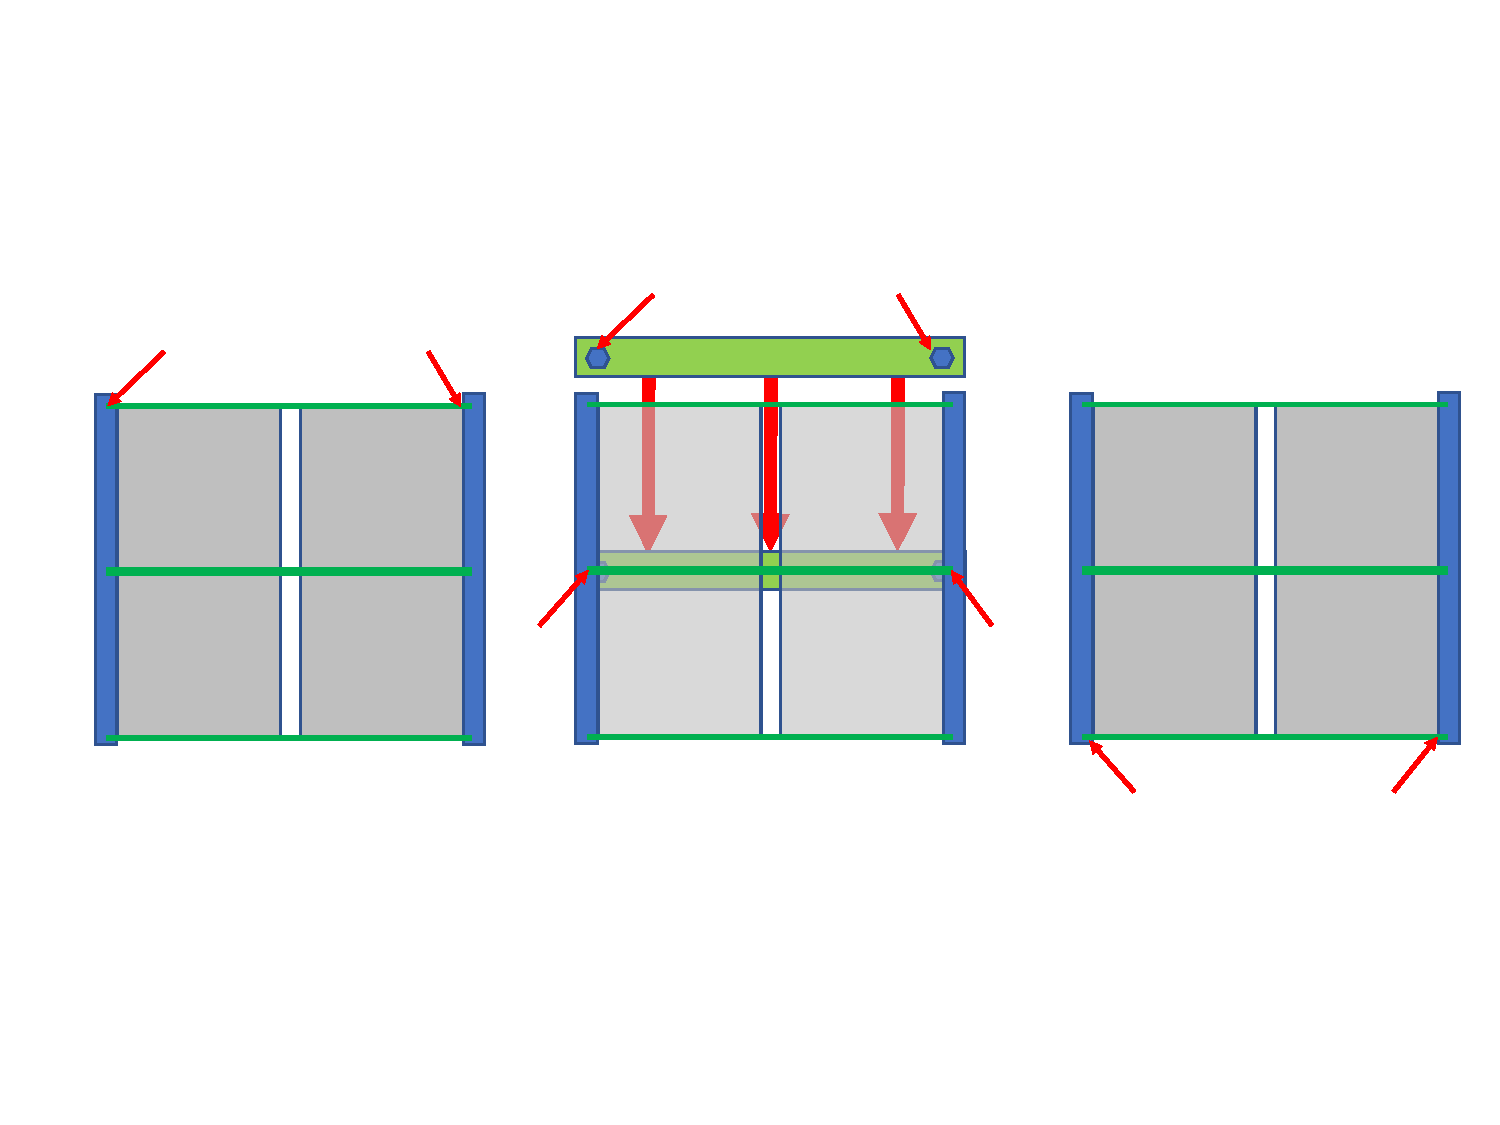
\includegraphics[width=0.8\textwidth]{dppd_reflective_panel_installation_sequence}
\end{dunefigure}

\subsection{Commissioning}
\label{subsec:dp-pds-commissioning}

The commissioning of the \dword{pds} is performed in partitions. The size of a single partition will be mainly determined by the \dword{daq} and the \dword{hv} systems. The \dword{daq} and \dword{hv} partitions are commissioned, including the relevant control systems, before the \dwords{pmt} are connected to these systems.

The exact availability of the cryostat as a sufficiently dark environment depends on the overall installation schedule. Once it is possible, the \dwords{pmt} are powered up, and basic functionality and performance checks are carried out. These include pedestal data taking, i.e., recording event data with external periodic triggering, and tests with the calibration system where the data taking is triggered in synchronization with a light source, as described in Section \ref{sec:dp-pds-calibration}.

Basic performance characteristics of the \dwords{pmt}, e.g., the dark count rate and gain, will be validated with the commissioning tests. Issues related to installation can then be identified and eliminated. A commissioned sector becomes a part of the overall detector and can join the global calibration data taking and commissioning.


